\documentclass[11pt, twocolumn]{article}

\usepackage{amsmath}
\usepackage{amssymb}
\usepackage{graphicx}

\begin{document}
\title{The Effectiveness of Brightness Metrics for Ball Detection}
\author{Marcus Christiansen, Will Gantt}
\maketitle

\abstract{Broadly, the goal of this project was to determine whether brightness measurements could be an effective tool for ball detection. Specifically, we considered how such metrics might be incorporated into the spot filter; first, in the identification of blacks spots, and, second, in a comparison between the brightness values of the top and bottom hemispheres of the ball itself. [State conclusion.]}
\section{Overview}
Since RoboCup's decision last year to replace the traditional orange ball with one more reminiscent of a classical soccer ball, teams have been faced with a slew of new vision challenges. As the ball's primary color is now white, teams must implement additional measures to distinguish it from other white objects, including field lines, goal posts, and robots. Furthermore, they must differentiate the black pentagons of the ball from chimeras like robot joints and other dark spots on the field. Thus, color alone can no longer serve as a reliable marker. Consequently, the Northern Bites have implemented a variety of additional checks. These include a determination of the expected radius of the ball at different locations on the field, an evaluation of the spatial relationships between black spots, and more obvious checks to verify that a candidate ball is in fact on the field. \\
\indent Although the ball detector concerns itself to a great extent with white and black, it makes almost no use of brightness inputs. Since black is notoriously difficult to characterize strictly on the basis of color (U and V) values, we wished to see whether brightness (the Y image) could provide some helpful information in this regard. 
\section{Experiment}
Currently, robots identify candidate balls using a spot filter. The basic principle consists in scanning an image with a ``filter,'' which comprises a small, square-shaped region nested within a larger one. At each position in the scan, the filter performs a simple check to determine whether the outer region is whiter on average than the inner one. The idea is that a ball will tend to be darker in the middle, since the black spots typically fall closer to its center, and whiter around the edges. [Include a graphic?] \\
The tests we ran operated on spots that the detector already identified. That is, they were intended to filter candidate balls rather than discover them. The first test considered the median Y-value of each detected black spot, with the goal of determining whether there was any consistent, significant difference between true positives (black spots actually on the ball) and false positives. The second compared the median Y-values of the top and bottom halves of the inner region of a white spot (a candidate ball). We reasoned that, because the field is lit from above, the top half of a ball should tend to be brighter than the bottom half. By the same logic, we hypothesized that the shadow cast by the ball on the field itself should mean that the area of the field directly below the ball will be darker than the area directly above it. This was implemented as a third test. \\
\indent All three tests were conducted on the same data, which comprised sets of logs taken in the robotics lab at levels of illumination of 150, 300, and 450 lux.\footnote{In truth, measuring the brightness of an entire room with this level of accuracy is impossible, given imperfections in the light meter, as well as minor fluctuations in the room itself. These values should therefore be taken as approximate.} For each level of brightness, we placed the robot in 12 different scenarios. For each scenario, we made adjustments to some combination of the following variables:
\begin{itemize}
\item The presence of the ball on the field (i.e., \emph{whether} it was on the field.)
\item The robot's distance from the ball.
\item The ball's position on the field.
\item The robot's position on the field.
\item The number of other robots present on the field.
\end{itemize}
Describe true/false positive differentiation.
\section{Results}

\indent Results of first test \\
\indent Results of second test \\
\indent Results of third test \\
Methodological problems:
\begin{itemize}
\item Lux values not exact (assuming we find no good evidence that there is a significant difference in brightness values between true and false positives, though, this shouldn't matter).
\item Would have been ideal to test in different locations, but again (given the presumptive results), this shouldn't matter.
\item With more time, we perhaps could have thought of more ways to reduce false positives.
\end{itemize}
\section{Future Work}
\begin{figure}
\begin{center}
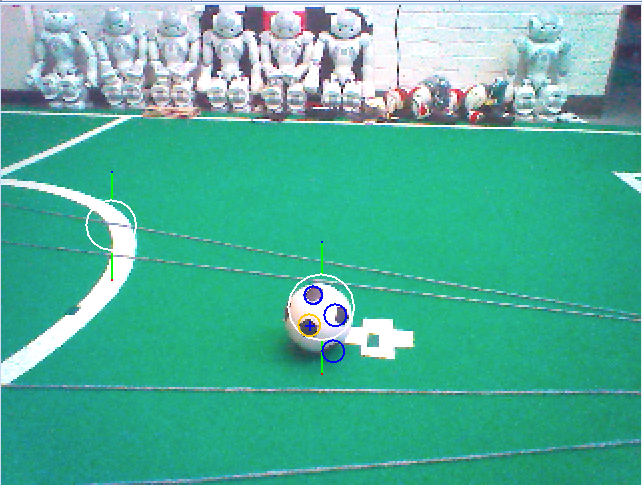
\includegraphics[scale=0.3]{s1.png}
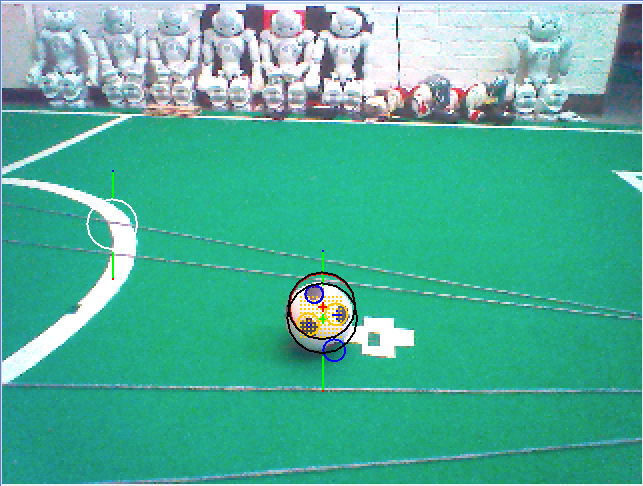
\includegraphics[scale=0.3]{s2.png}
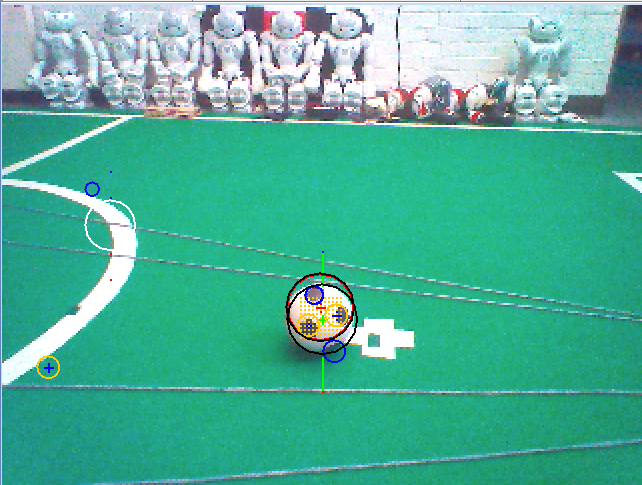
\includegraphics[scale=0.3]{s3.png}
\end{center}
\caption{Three logs}
\end{figure}
\begin{itemize}
\item Fragility of the filter; nearly identical logs can yield different results
\item Take only top 3 black spots; we got more than 3 on a number of the logs
\end{itemize}
\section{Conclusion}
\begin{itemize}
\item Restate purpose of experiment.
\item Summarize how experimented was carried out.
\item Summarize results.
\item Discuss how these results should influence future RoboCup research. (It seems that trying to characterize black is a futile exercise.)
\end{itemize}
\end{document}